\section{Detector Resolution Unfolding}
\label{sec:Unfolding}

Unfolding constants are derived from signal MC sample ($W\gamma\rightarrow\mu\nu_{\mu}\gamma$/$W\gamma\rightarrow{e}\nu_{e}\gamma$) with D'Agostini method using RooUnfold package [REFERENCE]\\

Unfolding stands for detector resolution only.\\

Migration matrix (Fig. \ref{fig:migrMatrices_Wg}) which is passed to RooUnfold is prepared the following way:
\begin{itemize}
  \item in fully selected signal MC sample, each event has a reconstructed level photon with $P_T^{\gamma(reco)}$ and matched generator level photon with $P_T^{\gamma(gen)}$
  \item $i_r$ - bin number determined by $P_T^{\gamma(reco)}$, $i_g$ - bin number determined by $P_T^{\gamma(gen)}$
  \item element $M_{i_g,i_r}$ of a migration matrix is weighted number of events in corresponding $[P_T^{\gamma(gen)},P_T^{\gamma(reco)}]$ bin
\end{itemize}

Response matrix (Fig. \ref{fig:respMatrices_Wg}) is a migration matrix normalized to each $i_r$ bin.\\
$N^{reco}_j = R_{ji} N^{gen}_i$\\

In data, we only have $N^{reco}_j$ which is our $P_T^{\gamma}$ spectrum fully selected and background subtracted. Using $R_{ji}$ determined by signal MC, it is needed to determine $N^{truth}_i$ in data now. Inversion method inverts $R_{ji}$ to determine $N^{truth}_i$.\\

After $P_T^{\gamma}$ spectrum is unfolded, measurements in different $P_T^{\gamma}$ bins are no longer independent. RooUnfold provides a covariance matrix.\\

A correlation matrix (Fig. \ref{fig:corrMatrices_Wg}) is derived from covariance matrix as:
$M^{corr}_{ij} = \frac{C_i \cdot C_j}{\sqrt{(C_{ii} \cdot C_{jj})}} $ where $C_{ij}$ is a matrix element of a covariance matrix.\\

%Checked that D'Agostini and simple inversion matrix give the same result (yields are the same, errors are different). Also checked that privately implemented unfolding gives the same result as RooUnfold. Also the MC closure test is routinely performed every time when unfolding is applied on data. \\
%Migration 
%TODO: switch to more recent version of RooUnfold\\
%TODO: present table: data yields; unfolded data yields; MC yeidls; unfolded MC yields; gen MC yields\\
%TODO: think whether additional eff reco is needed here\\
%Unfolding recommendations for SMP \\

\begin{figure}[htb]
  \begin{center}
   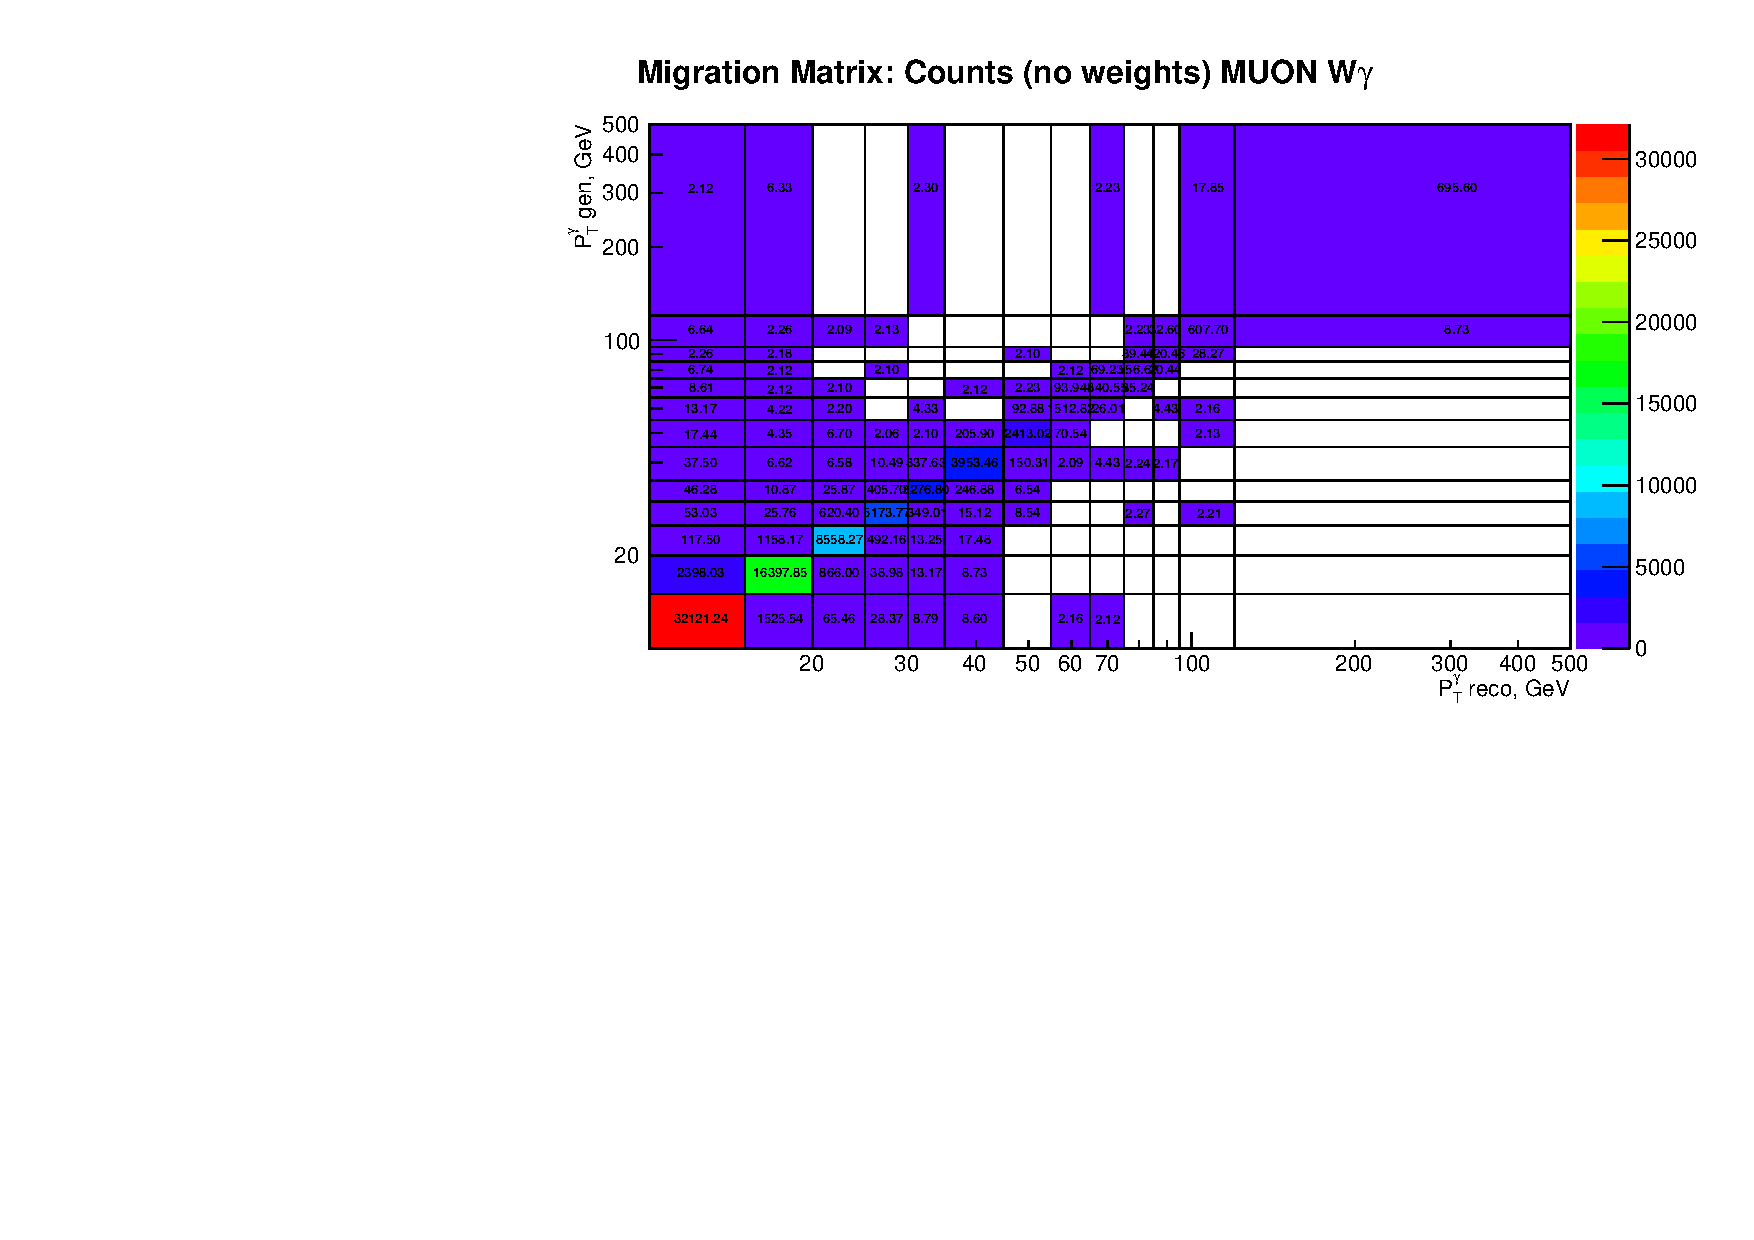
\includegraphics[width=0.90\textwidth]{figs_v11/MUON_WGamma/Constants/cMigrMatrix_MUON_WGamma__yield_pm_stat.pdf}\\
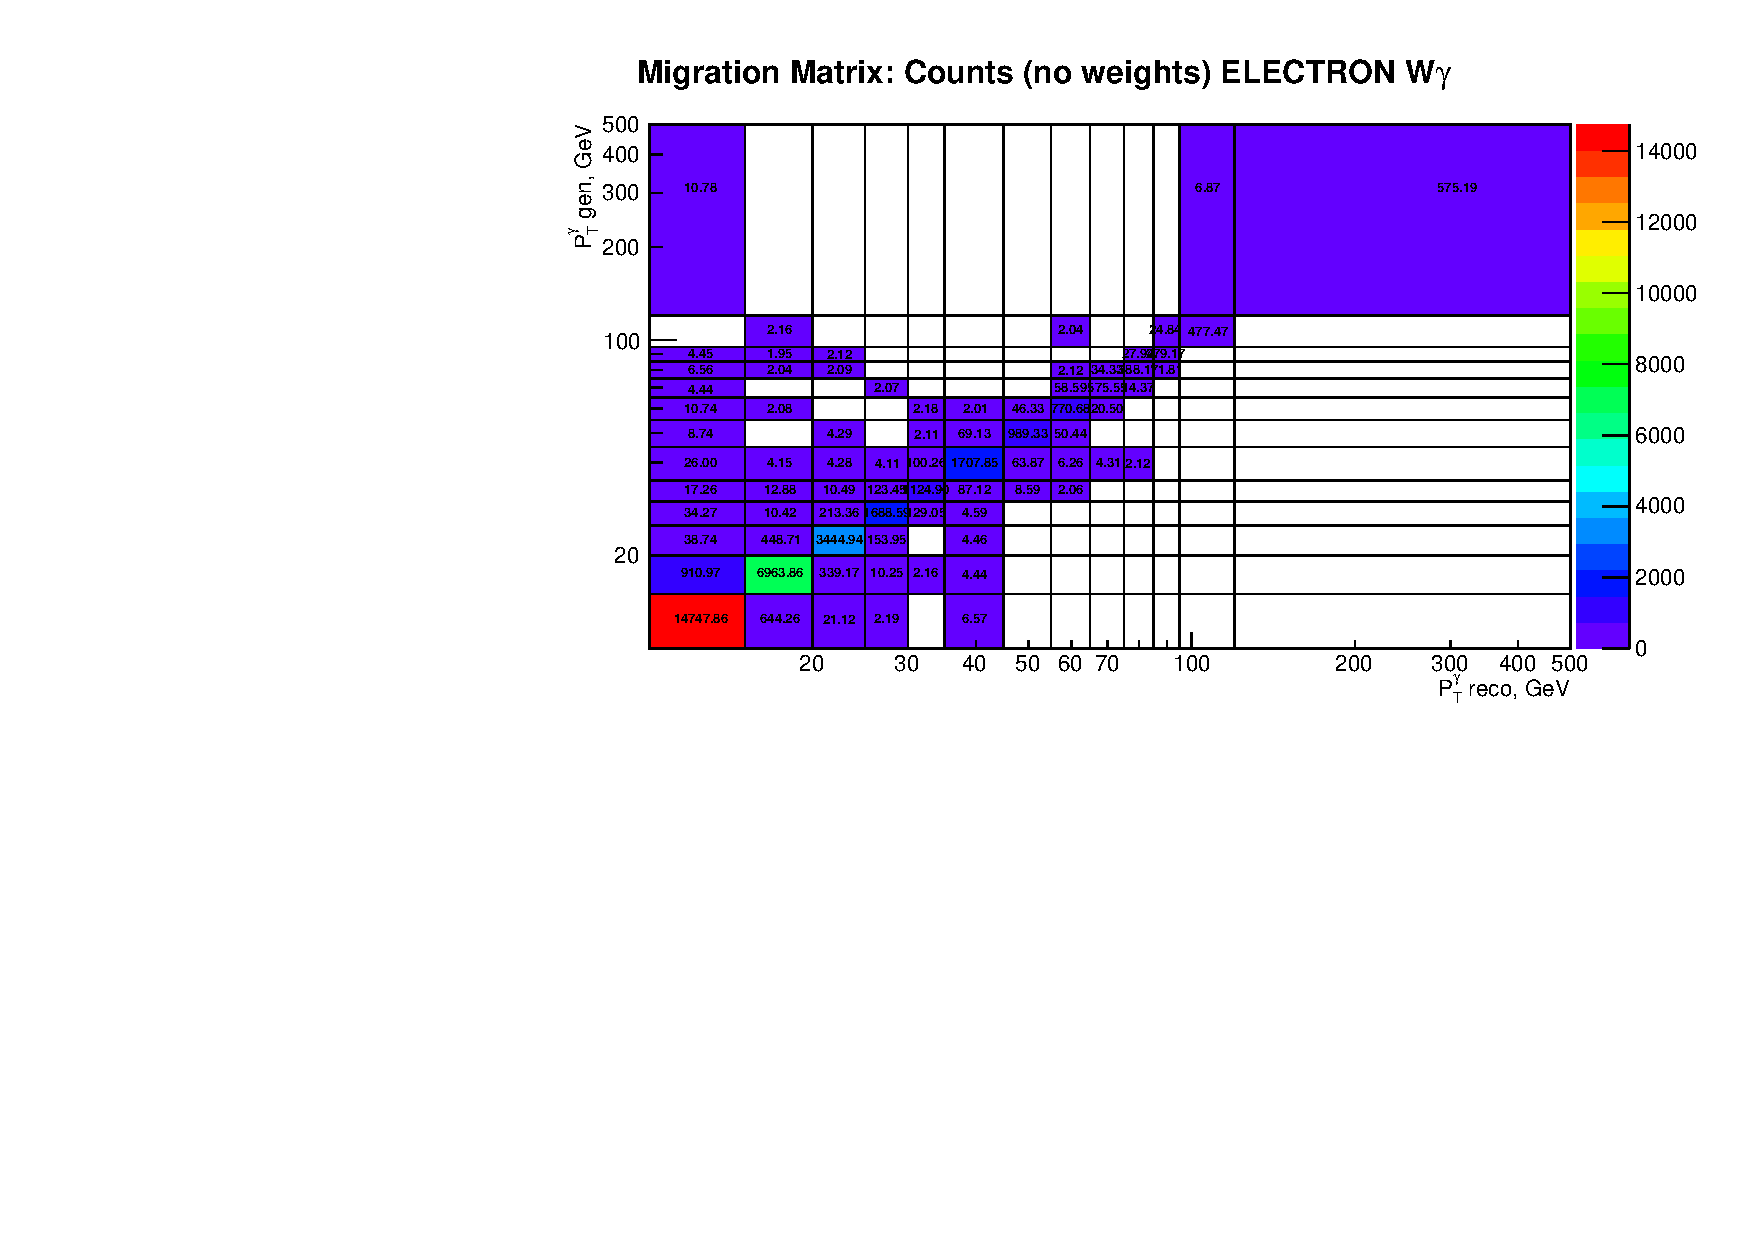
\includegraphics[width=0.90\textwidth]{figs_v11/ELECTRON_WGamma/Constants/cMigrMatrix_ELECTRON_WGamma__yield_pm_stat.pdf}
  \caption{Migration matrix derived from signal MC with matrix inversion method.}
  \label{fig:migrMatrices_Wg}
  \end{center}
\end{figure}

\begin{figure}[htb]
  \begin{center}
   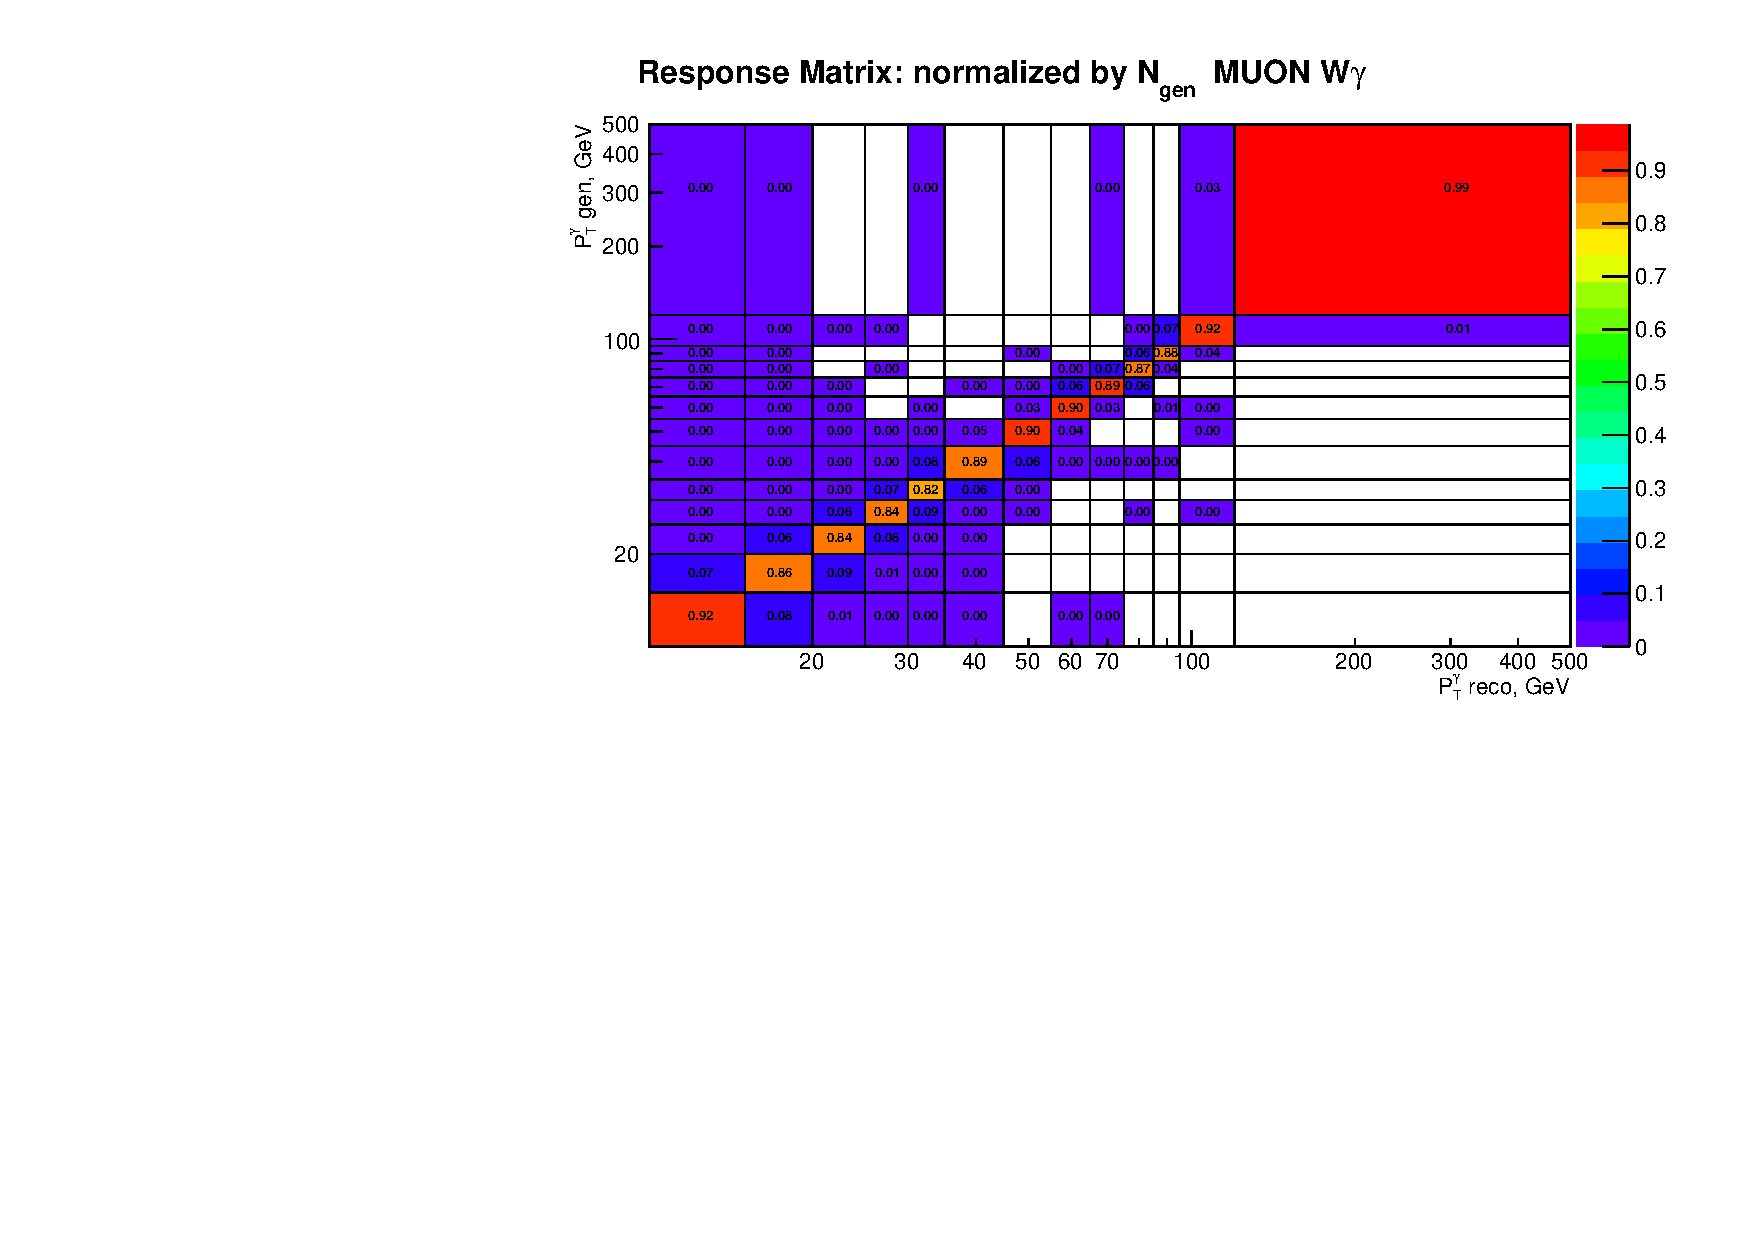
\includegraphics[width=0.90\textwidth]{figs_v11/MUON_WGamma/Constants/cResponseMatr_MUON_WGamma__yield_pm_stat.pdf}\\
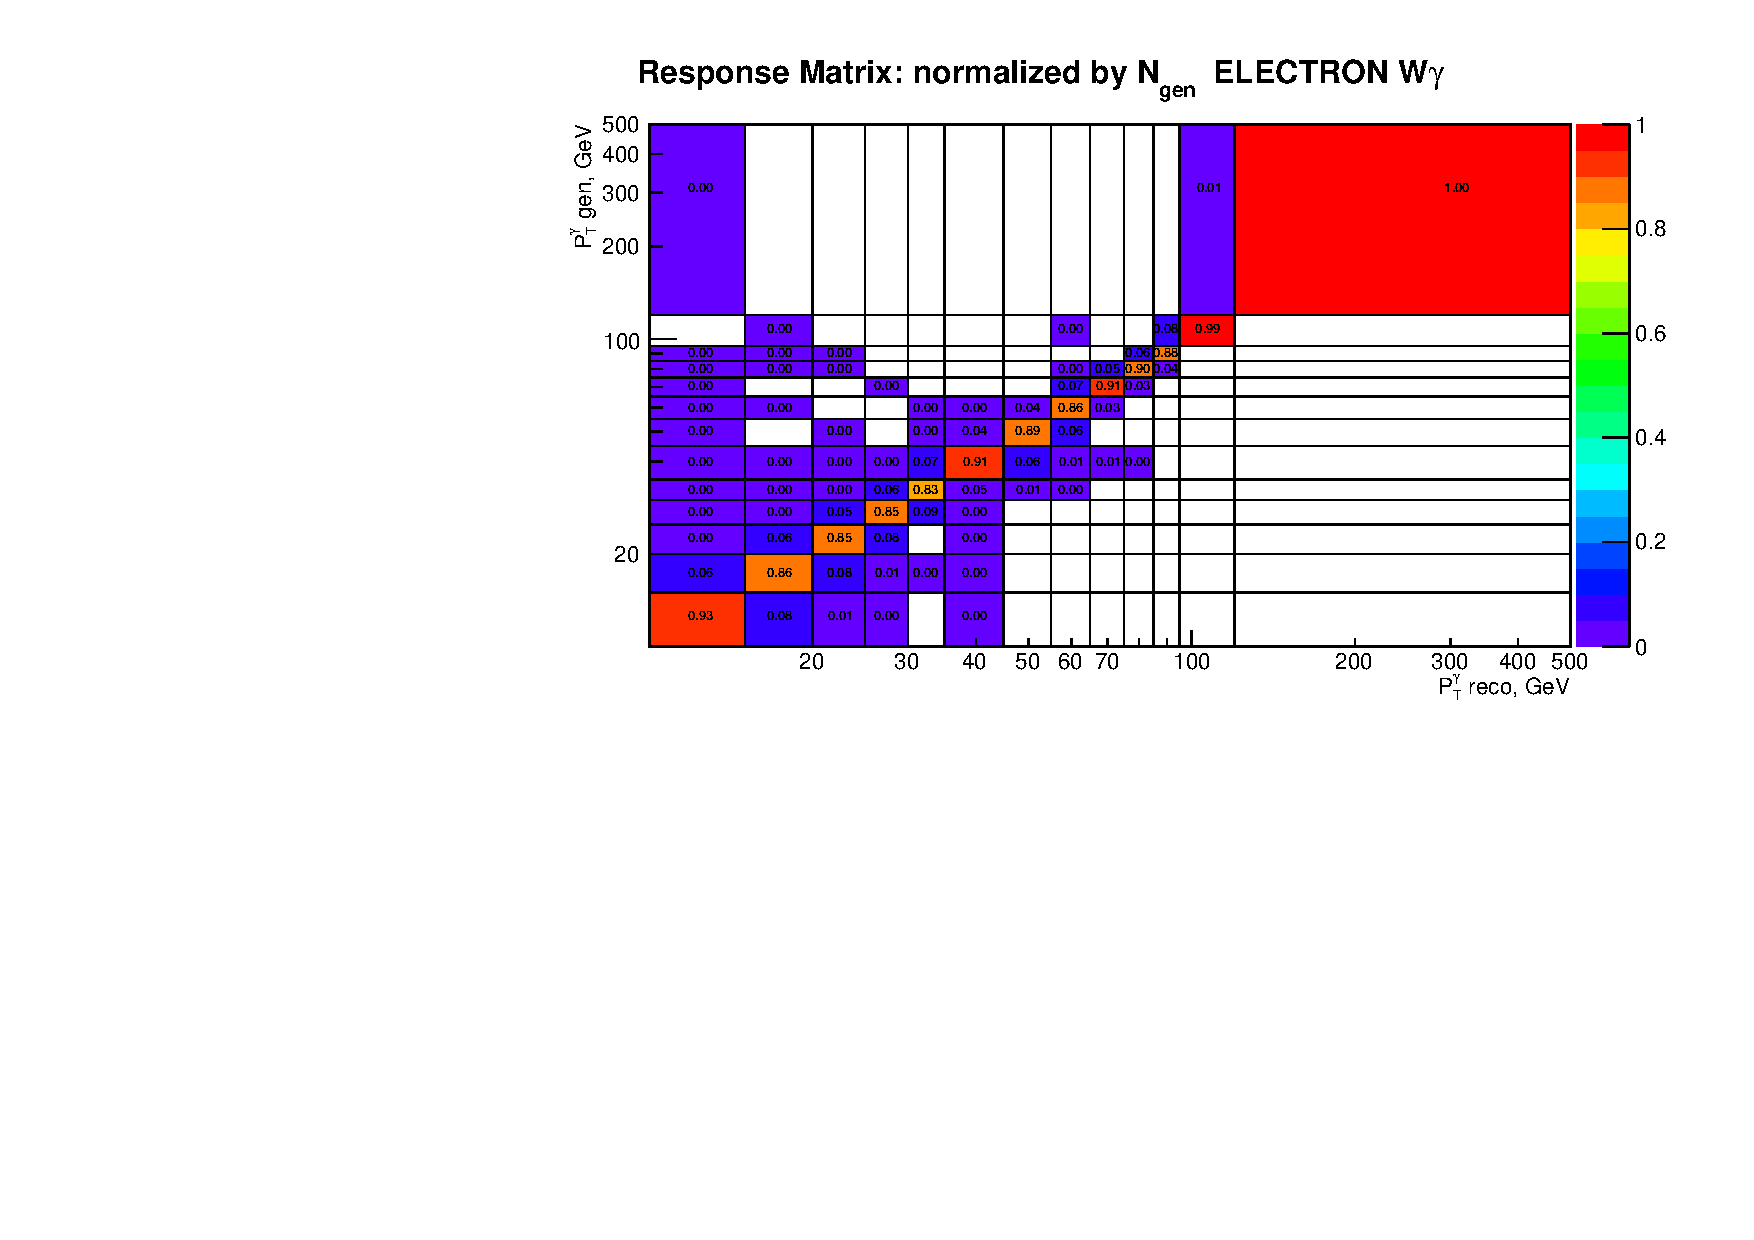
\includegraphics[width=0.90\textwidth]{figs_v11/ELECTRON_WGamma/Constants/cResponseMatr_ELECTRON_WGamma__yield_pm_stat.pdf}
  \caption{Response matrix derived from signal MC with matrix inversion method.}
  \label{fig:respMatrices_Wg}
  \end{center}
\end{figure}

\begin{figure}[htb]
  \begin{center}
   \includegraphics[width=0.90\textwidth]{figs_v11/MUON_WGamma/Constants/matrCorrelation_yield_pm_stat.pdf}\\
\includegraphics[width=0.90\textwidth]{figs_v11/ELECTRON_WGamma/Constants/matrCorrelation_yield_pm_stat.pdf}
  \caption{Correlation Matrices as provided by RooUnfold right after unfolding is applied.}
  \label{fig:corrMatrices_Wg}
  \end{center}
\end{figure}

%[1] https://indico.cern.ch/event/322577/ 
%[2] https://twiki.cern.ch/twiki/bin/view/CMS/TwikiSMP-GENRecommendations\#Unfolding\_How\_to

The results of the MC closure check are summarized in Tab. \ref{tab:unf_mc_closure_MUON_WGamma}-\ref{tab:unf_mc_closure_ELECTRON_WGamma} for the muon and electron channels respectively. Gen-level and rec yields in the tables are generator level and reconstructed $P_T^{\gamma}$ yields in the signal MC. Then reconstructed yields are smeared with Gaussian according to the errors on the yields. Then the Matrix Inversion and D'Agostini unfoldings are applied using RooUnfold. The unfolded yields with any method show reasonable agreement to the gen-level yields except the underflow bin (10-15 GeV). The disagreement in the underflow bin may be due to events with $P_T^{\gamma}<10$ GeV which are not available. \\ 

\begin{table}[h]
  \scriptsize
  \begin{center}
  \caption{Unfolding, MC closure test. MUON WGamma}
  \begin{tabular}{|c|c|c|c|c|}
  bin &  yields &   yields &  unfolded &  unfolded \\ \hline
   limits &  gen-level & rec &  inversion &  D'Agostini \\ \hline
10 -  15 &     $33888\pm 273$ &     $37074\pm 286$ &     $36226\pm206$ &     $36222\pm204$ \\ \hline
 15 -  20 &     $19736\pm 207$ &     $19181\pm 203$ &     $19612\pm171$ &     $19619\pm169$ \\ \hline
 20 -  25 &     $10364\pm 149$ &     $10171\pm 148$ &     $10358\pm122$ &     $10354\pm119$ \\ \hline
 25 -  30 &     $6254\pm 116$ &     $6156\pm 115$ &     $6233\pm96$ &     $6234\pm96$ \\ \hline
 30 -  35 &     $4026\pm  93$ &     $4007\pm  93$ &     $4010\pm81$ &     $4010\pm78$ \\ \hline
 35 -  45 &     $4516\pm  99$ &     $4461\pm  98$ &     $4502\pm79$ &     $4502\pm79$ \\ \hline
 45 -  55 &     $2731\pm  77$ &     $2680\pm  76$ &     $2724\pm57$ &     $2724\pm60$ \\ \hline
 55 -  65 &     $1662\pm  60$ &     $1686\pm  61$ &     $1655\pm45$ &     $1655\pm46$ \\ \hline
 65 -  75 &     $987\pm  46$ &     $945\pm  45$ &     $979\pm38$ &     $979\pm35$ \\ \hline
 75 -  85 &     $659\pm  38$ &     $638\pm  37$ &     $654\pm30$ &     $653\pm30$ \\ \hline
 85 -  95 &     $495\pm  33$ &     $480\pm  32$ &     $489\pm27$ &     $489\pm25$ \\ \hline
 95 - 120 &     $664\pm  38$ &     $663\pm  38$ &     $661\pm28$ &     $661\pm28$ \\ \hline
120 - 500 &     $726\pm  40$ &     $704\pm  39$ &     $720\pm26$ &     $720\pm27$ \\ \hline
500 - 2000 &     $2\pm   2$ &     $2\pm   2$ &     $2\pm1$ &     $2\pm1$ \\ \hline
  \end{tabular}
  \label{tab:unf_mc_closure_MUON_WGamma}
  \end{center}
\end{table}

\begin{table}[h]
  \scriptsize
  \begin{center}
  \caption{Unfolding, MC closure test. ELECTRON WGamma}
  \begin{tabular}{|c|c|c|c|c|}
  bin &  yields &   yields &  unfolded &  unfolded \\ \hline
   limits &  gen-level & rec &  inversion &  D'Agostini \\ \hline
 10 -  15 &     $16025\pm 185$ &     $16849\pm 190$ &     $17117\pm143$ &     $17116\pm141$ \\ \hline
 15 -  20 &     $8246\pm 131$ &     $8111\pm 130$ &     $8194\pm109$ &     $8196\pm108$ \\ \hline
 20 -  25 &     $4093\pm  92$ &     $4046\pm  92$ &     $4083\pm75$ &     $4082\pm74$ \\ \hline
 25 -  30 &     $2080\pm  66$ &     $1987\pm  64$ &     $2072\pm55$ &     $2072\pm55$ \\ \hline
 30 -  35 &     $1387\pm  54$ &     $1361\pm  54$ &     $1378\pm47$ &     $1378\pm46$ \\ \hline
 35 -  45 &     $1925\pm  64$ &     $1886\pm  63$ &     $1915\pm51$ &     $1915\pm50$ \\ \hline
 45 -  55 &     $1124\pm  49$ &     $1108\pm  48$ &     $1116\pm37$ &     $1116\pm38$ \\ \hline
 55 -  65 &     $855\pm  42$ &     $892\pm  43$ &     $848\pm33$ &     $848\pm34$ \\ \hline
 65 -  75 &     $655\pm  38$ &     $635\pm  37$ &     $649\pm30$ &     $649\pm28$ \\ \hline
 75 -  85 &     $447\pm  32$ &     $433\pm  32$ &     $442\pm24$ &     $442\pm24$ \\ \hline
 85 -  95 &     $316\pm  27$ &     $316\pm  27$ &     $311\pm21$ &     $311\pm20$ \\ \hline
 95 - 120 &     $507\pm  34$ &     $484\pm  33$ &     $501\pm23$ &     $501\pm23$ \\ \hline
120 - 500 &     $593\pm  37$ &     $575\pm  36$ &     $587\pm23$ &     $587\pm24$ \\ \hline
500 - 2000 &     $4\pm   3$ &     $4\pm   3$ &     $4\pm2$ &     $4\pm2$ \\ \hline
  \end{tabular}
  \label{tab:unf_mc_closure_ELECTRON_WGamma}
  \end{center}
\end{table}

%Comparison of the Inversion and d'Agostini methods on data.

%\begin{table}[h]
%  \scriptsize
%  \begin{center}
%  \caption{Unfolding on data. Stat. error. ELECTRON WGamma}
%  \begin{tabular}{|c|c|c|c|c|c|}
%Yields & sign. MC & sign. MC & data & data unf. & data unf.\\
%       & gen-level & rec.    & input & inversion & D'Agostini\\ \hline
%  \label{tab:unf_data_ELECTRON_WGamma}
%  \end{center}
%\end{table}

%\begin{table}[h]
%  \scriptsize
%  \begin{center}
%  \caption{Unfolding on data. Stat. error. MUON WGamma}
%  \begin{tabular}{|c|c|c|c|c|c|}
%Yields & sign. MC & sign. MC & data & data unf.& data unf.\\
%       & gen-level & rec.    & input & inversion & D'Agostini\\ \hline
%  \end{tabular}
%  \label{tab:unf_data_MUON_WGamma}
%  \end{center}
%\end{table}
